\documentclass[10pt,twocolumn,letterpaper]{article}

\usepackage{cvpr}
\usepackage{times}
\usepackage{epsfig}
\usepackage{graphicx}
\usepackage{amsmath}
\usepackage{amssymb}

% Include other packages here, before hyperref.

% If you comment hyperref and then uncomment it, you should delete
% egpaper.aux before re-running latex.  (Or just hit 'q' on the first latex
% run, let it finish, and you should be clear).
\usepackage[breaklinks=true,bookmarks=false]{hyperref}

\cvprfinalcopy % *** Uncomment this line for the final submission

\def\cvprPaperID{0000} % *** Enter the CVPR Paper ID here
\def\httilde{\mbox{\tt\raisebox{-.5ex}{\symbol{126}}}}

% Pages are numbered in submission mode, and unnumbered in camera-ready
%\ifcvprfinal\pagestyle{empty}\fi
\setcounter{page}{1}
\begin{document}
	
	%%%%%%%%% TITLE
	\title{A Review and a few modifications on Metric Learning Methods}
	
	\author{First Author\\
		Institution1\\
		Institution1 address\\
		{\tt\small firstauthor@i1.org}
		% For a paper whose authors are all at the same institution,
		% omit the following lines up until the closing ``}''.
		% Additional authors and addresses can be added with ``\and'',
		% just like the second author.
		% To save space, use either the email address or home page, not both
		\and
		Second Author\\
		Institution2\\
		First line of institution2 address\\
		{\tt\small secondauthor@i2.org}
	}
	
	\maketitle
	%\thispagestyle{empty}
	
	%%%%%%%%% ABSTRACT
	\begin{abstract}
		Metric learning is the task of learning a distance function on pair of objects. We review three metric learning methods based on deep learning, including Siamese Network, Triplet Network and n-Tuple Network framework. These frameworks output low dimensional embedding for input data, on which we may use Euclidean distance as the distance function. These frameworks all include a set of neural networks sharing the same structure and parameters and a loss function combining the outputs of the networks. In this work, we wrote a wrapper class for the network to hide the low-level implementation, and focus on the design of the high-level frameworks and loss functions. In our experiment on MNIST dataset and a classic network structure, Siamese Network has a mediocre performance while Triplet Network produces better embeddings. We are not able to make the original n-Tuple Network work. However, we have tested a few modified versions of it, which keep the framework unchanged but use different loss functions.
	\end{abstract}
	
	%%%%%%%%% BODY TEXT
	\section{Introduction}
	Metric learning is the task of learning a distance function on pair of objects. The most trivial definition of distance of two instances (which can be two images, two sequences, etc.) is the Euclidean distance. However, Euclidean distance may not be a good indicator for specialized tasks, because it cannot represent the intrinsic structure of the data. Theoretically, many high dimensional datasets can be viewed as low dimensional manifold embedded in a high dimensional space, where Euclidean distance cannot capture the manifold.
	
	To solve this problem, many Metric learning algorithms are invented. The classical ones include Isomap, Locally Linear Embedding (LLE), Stochastic Neighbor Embedding, etc. These methods are all unsupervised methods. In the deep learning area, Raia Hadsell et~al. have introduced Siamese Network \cite{hadsell2006dimensionality}, which can be viewed as a framework including two neural networks of the same structure and sharing the same parameters and a loss function defines on the two outputs and the labels of the two inputs. Commonly, the loss function call for a small distance of the outputs when the two inputs are of the same label and vice versa. Elad Hoffer and Nir Ailon have invented Triplet Network \cite{DBLP:journals/corr/HofferA14}, which is an extension of Siamese Network, but includes three networks. The Triplet Network processes two instances from one class and one instance from another class at the same time. n-Tuple Network \cite{sohn2016improved} further generalize the idea of Triplet Network, where two instances from one class and multiple instances from the other classes are used at one time.\\
	
	In section \ref{sec:mech} we show the mechanisms of the aforementioned deep learning methods in detail. Some important details about implementation is shown in section \ref{sec:Impl}. We show our experiments in and discusses the results in section \ref{sec:Res}. The conclusion is in section \ref{sec:Conc}\\
	
	We use two laptops to perform the experiments. One of them is equipped with Intel Core i7 5700HQ and NVidia 960M graphics. Another one has Intel Core i7-6500U and NVidia 940M GPU.
	
	\section{Mechanisms \label{sec:mech}}
		\subsection{Siamese Network}
			Siamese Network is a framework for metric learning. The structure is shown in figure \ref{fig:siamese_struct}.
			
			\begin{figure}[htbp]
				\begin{center}
					%\fbox{\rule{0pt}{2in} \rule{0.9\linewidth}{0pt}}
					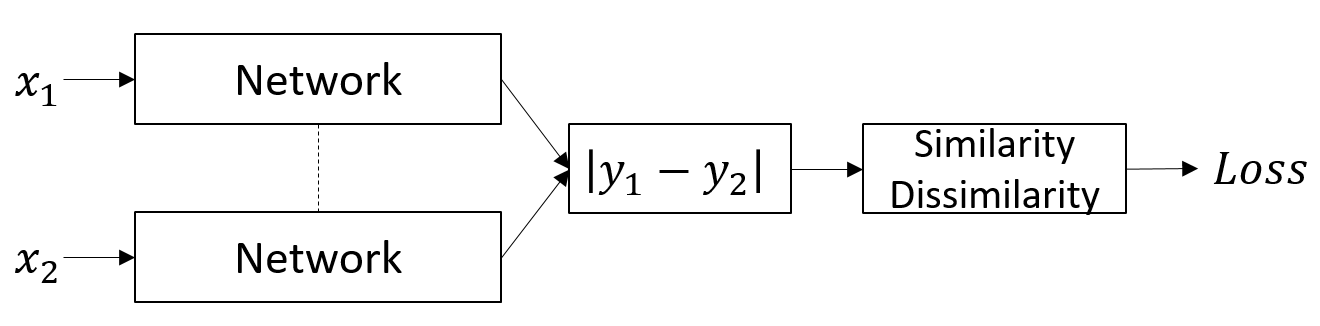
\includegraphics[width=0.9\linewidth]{siamese_struct}
				\end{center}
				\caption{Structure of Siamese Network.\label{fig:siamese_struct}}
			\end{figure}
			
			It contains two parts, the twin networks (In fact its name ``Siamese'' is related to twin) and the loss function. The structure of the framework is shown in figure ???. Each one of the twin networks takes one instance from the dataset, denoted as $x_1$ and $x_2$, and output the result 
			\begin{equation}
				y_1 = Net(x_1);\; y_2 = Net(x_2)
			\end{equation}
			respectively. The loss function is defined as follows. \footnote{Expressions are slightly different from the original paper to keep consistent through our article.}
			\begin{equation}
				Loss = (1-S)L_S(\lvert y_1 - y_2 \rvert) + S L_D(\lvert y_1 - y_2 \rvert)
			\end{equation}
			where $L_S(\bullet)$ and $L_D(\bullet)$ stands for loss functions for similarity and dissimilarity respectively. When $x_1$ and $x_2$ are in the same class (or is similar on some perspective), label $S$ is set to be $1$, and the loss is caused by dissimilarity. When $x_1$ and $x_2$ are not in the same class, $Y$ is set to $0$ and gives a penalty on similarity. The formal definitions of the functions are as follows.

			\begin{equation}
				L_S = \frac{1}{2}\lvert y_1 - y_2 \rvert^2
			\end{equation}
			\begin{equation}
				L_D = \frac{1}{2}\{max(0, m-|y_1-y_2|)\}^2 \label{eq:negative}
			\end{equation}
			where $m$ is a positive parameter. Generally speaking, $L_D$ treats two points whose distance is more than $m$ as totally separated and puts no penalty on them.
			
			When training using batches, we may simply average the loss function of several runs.
		\subsection{Triplet Network}
			Triplet Network is a enhanced version of Siamese Network, which processes similar instance and dissimilar instance at the same time. The structure of the framework is shown in figure \ref{fig:triplet_struct}. The loss function is not just the similarity or dissimilarity, but is based on comparison of the similarity of similar instances and dissimilarity of dissimilar instances. 
			
			\begin{figure}[htbp]
				\begin{center}
					%\fbox{\rule{0pt}{2in} \rule{0.9\linewidth}{0pt}}
					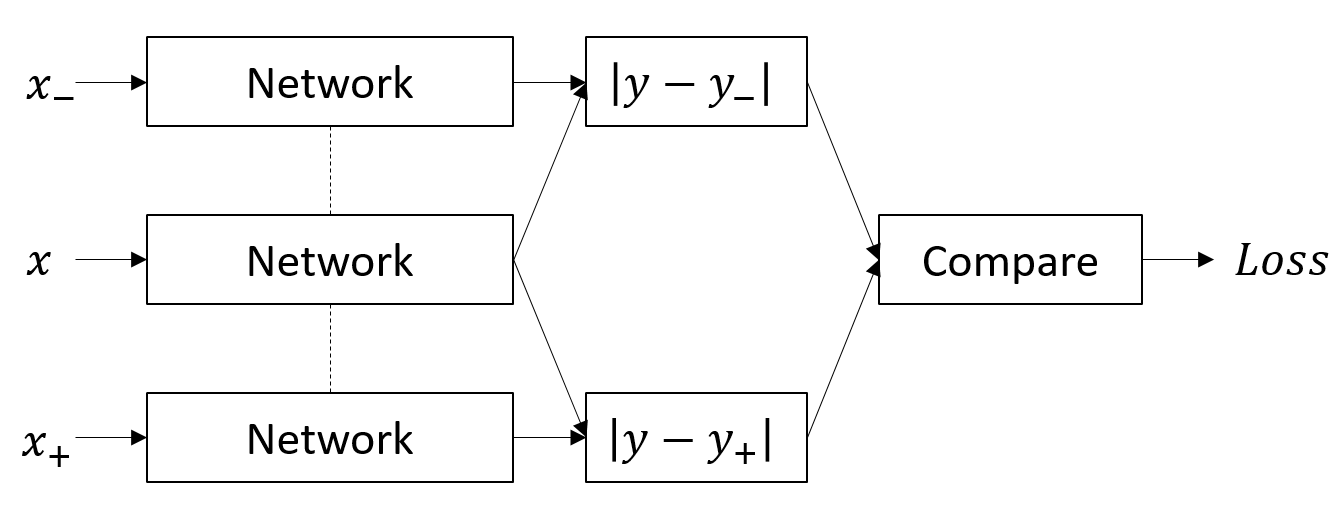
\includegraphics[width=0.9\linewidth]{triplet_struct}
				\end{center}
				\caption{Structure of Triplet Network.\label{fig:triplet_struct}}
			\end{figure}
			
			The framework takes three instances as input at one time. However, contrast with Siamese Network, the instances are not chosen totally randomly. Instead, we first choose one instance $x$ randomly, and then choose one instance $x_+$ from the same class as the positive example. Finally, we choose $x_-$ from another classes as the negative example. Three instances are fed to the network at one time and this is the origin of the name ``Triplet''. The output of the three instances are denoted as
			\begin{equation}
				y = Net(x);\; y_+ = Net(x_+);\; y_-=Net(x_-)
			\end{equation}
			
			Formally, the loss function is defined as
			\begin{equation}
				Loss = \lvert(d_+, d_--1)\rvert^2 = const\bullet d_+^2
			\end{equation}
			where $d_+$ and $d_-$ are the normalized exponential distance, defined as follows.
			\begin{equation}
				d_+ = \frac{\exp{(\lvert y-y_+ \rvert)}}{\exp{(\lvert y-y_+ \rvert)} + \exp{(\lvert y-y_- \rvert)}}
			\end{equation}
			and
			\begin{equation}
				d_- = \frac{\exp{(\lvert y-y_- \rvert)}}{\exp{(\lvert y-y_+ \rvert)} + \exp{(\lvert y-y_- \rvert)}}
			\end{equation}
			This loss function call for a higher $\frac{\exp{(\lvert y-y_+ \rvert)}}{\exp{(\lvert y-y_+ \rvert)}}$ ratio, which means shorter distance for similar instances and longer distance for dissimilar instances.
			
			This framework can also use batched training by simply average the loss function over multiple triplets of input instances.
			
			\subsection{n-Tuple Network}

				As seem in the improvement Triplet Network is making, we can sample several negative examples for the training set, 
				$$(x,x^+,x^-_1,x^-_2,\cdots x^-_{n-1})$$
				But generating $M$ batches of samples like this requires lots of computation burden. So instead of generating $M\times(N+1)$ examples and calculate the loss on them, we generate $N$ pairs of images of the same type and distinct pairs of images are of different labels. And the corresponding $(N+1)-$pair loss is given by 
				\begin{equation}
				L(\{x_i,x_i^+\}^N_{i=1})=\frac{1}{N}\log(\sum_{i=1}^N\exp(\sum_{j=1}^Ny^T_iy_j^+-y_i^Ty_i^+))  \label{eq:n-pair}
				\end{equation}
				As observed in equation \ref{eq:n-pair}, if $\sum^N\limits_{i=1}\exp(y^T_iy_j^+-y_i^Ty_i^+)$ is negative then embeddings $\{C\cdot y_i,C\cdot y_i^+\}$ gives a lower loss with any negative constant $C$, thus restrictions on norm of embeddings are needed. The structure is shown in figure \ref{fig:tuple_struct}.
				
				\begin{figure}[htbp]
					\begin{center}
						%\fbox{\rule{0pt}{2in} \rule{0.9\linewidth}{0pt}}
						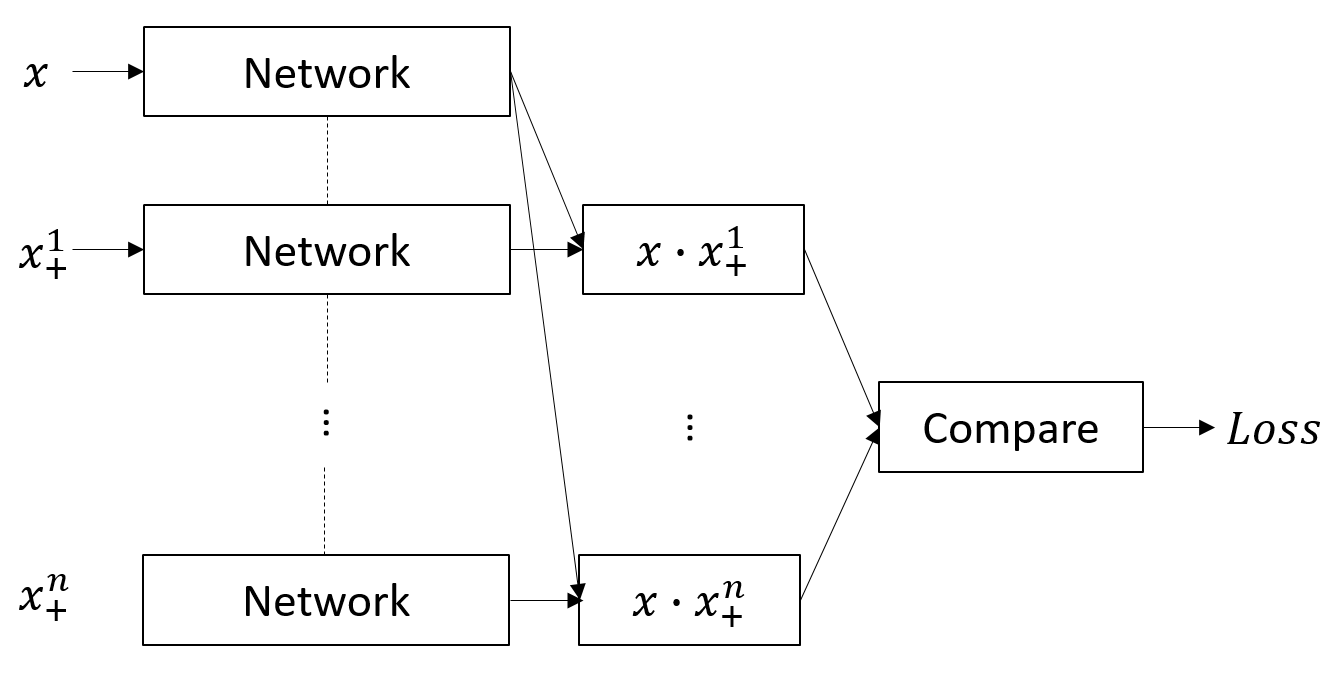
\includegraphics[width=0.9\linewidth]{tuple_struct}
					\end{center}
					\caption{Structure of Triplet Network.\label{fig:tuple_struct}}
				\end{figure}
				
				One characteristic of n-Tuple Network is that n-Tuple Network leverages dot product instead of Euclidean distance as the approach to measure the distance of two outputs, which is different from the other two frameworks.

	\section{Implementations \label{sec:Impl}}
		As is mentioned above, these frameworks integrate multiple networks sharing parameters into one framework. We have two ways to achieve this. We may implement multiple networks but using the same parameters. We may also use only one network, feed the network with one set of well-arranged instances and slice the outputs when calculating the loss functions. For Siamese Network and Triplet Network, the first one is easier to implement. However, for n-Tuple network, the second one is more compact.
	
		To facilitate our experiment, we write a wrapper class \verb|Network| for convolutional network, which provides three member functions \verb|add_conv()|, \verb|add_fc()| and \verb|connect()|. \verb|add_conv()| and \verb|add_fc()| are used to declare new convolutional layer or fully connected layer into the network, while \verb|connect()| takes an input placeholder and output an output tensor. It is very easy to implement a convolutional network with this class.
		
		For example, when we want to implement a convolutional network on MNIST dataset, which consists of images of $28 \times 28$ pixels and $1$ channel, and embed it to a 2 dimensional vector, we simply write
		\begin{verbatim}
			net = Network(28, 28, 1, 2)
		\end{verbatim}
		We use a modified version of the most common structure of network, i.e. two convolutional layers followed by one fully connected layers. The convolutional layers are declared by
		\begin{verbatim}
			net.add_conv(5, 5, 2, 2, 32)
			net.add_conv(5, 5, 2, 2, 64)
		\end{verbatim}
		which means two layers with $5\times 5$ convolutional kernels and $2\times 2$ max-pooling windows. The number of channels in output is $32$ and $64$ respectively.
		The fully connected layers is
		\begin{verbatim}
			net.add_fc(1024)
		\end{verbatim}
		which means a fully connected layer whose output has 1024 dimensions. The class will automatically flatten the data when we stop adding convolutional layer and start to add fully connected layer. (And throw exception if we try to add a convolutional layer after flattening.)
		
		Because our task is different from the original network for classification, we add one more fully connected layer into the network
		\begin{verbatim}
			net.add_fc(256)
		\end{verbatim}
		
		The dimensionality of data is handled by the class automatically so we do not need to  declare weight matrices manually and calculate their dimensionalities by hand.
		
		Then, we can write
		\begin{verbatim}
			output = net.connect(input)
		\end{verbatim}
		to finalize the network, in which output is the 2-dimensional output vector, while input is the placeholder to get input data. (The network will tacitly add a fully connected layer to further transform the 256-dimensional vectors into 2-dimensional vectors.)
		
		\subsection{Multiple Network Implementation}
			On one perspective, the frameworks includes multiple parallel networks, so we call \verb|connect()| multiple times to connect multiple networks. Use Triplet Network as an example, we connect three networks for the three inputs \verb|mid_input| $x$, \verb|pos_input| $x_+$ and \verb|neg_input| $x_-$.
			\begin{verbatim}
				mid_output = net.connect(mid_input)
				pos_output = net.connect(pos_input)
				neg_output = net.connect(neg_input)
			\end{verbatim}
			In practice, the three inputs are all batches of instances, and the loss function are defined as average of each triplet.
			
		\subsection{Single Network Implementation}
			On another perspective, the frameworks simply use one network to process all the inputs, and then separate the inputs into portions and define the loss function on them. Following this idea, we implement another version that only connect one network. We carefully arrange the input data, and slice the output data to rearrange the tuples.
			
			For example, we use 20 10-tuples in one batch, and each tuple includes 10 pairs instances, each of them is embedded to a 2-dimensional vector. We reshape the output as follows.
			\begin{verbatim}
				tf.reshape(output, [20, 10, 2, 2])
			\end{verbatim}
			Where the number 20, 10, 2 and 2 correspond to 20 tuples, 10-tuple, ``pair'' and 2-dimensional respectively.
	\section{Experiments and Discussions \label{sec:Res}}
		\subsection{Siamese Network}
			The result of siamese network is shown in figure \ref{fig:siamese}. The 10 digits are fairly separated. We can still find some substructure of output that can be indicated by the input data. For example, digits 9 is confused with digits 7 and digit 4 some times. Digit 2 and 3 also have a confusion area. This is a good result in a sense because it is reasonable to see a shorter distance from ``9'' to ``7'' than from ``9'' to ``8'' based on their appearance.
			\begin{figure}[htbp]
				\begin{center}
					%\fbox{\rule{0pt}{2in} \rule{0.9\linewidth}{0pt}}
					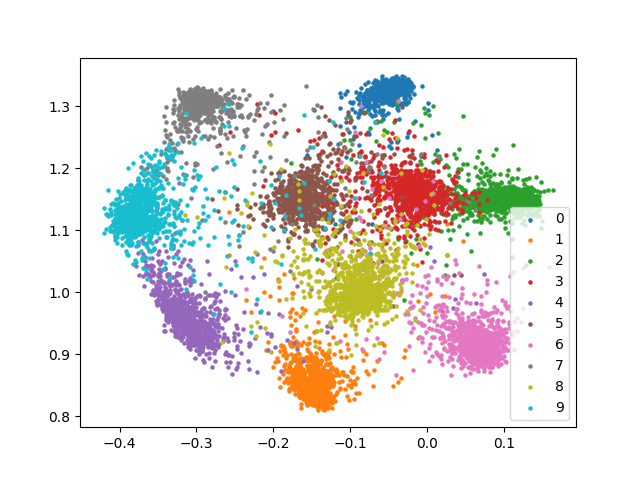
\includegraphics[width=0.9\linewidth]{siamese}
				\end{center}
				\caption{Result of Siamese Network. The separation is fair. Some interesting substructure is notable (digit 4, 7 and 9; digit 2 and 3).\label{fig:siamese}}
			\end{figure}
			
			The ratio of positive example to negative example is $10:45$ in this first try. We have test on different ratio to evaluate the importance of positive examples and negative examples. In particular, we use a ratio of $450:45$. The performance is greatly impaired, which is shown in figure \ref{fig:siamese_more_pos}. Digit ``2'', ``3'', ``5'' and ``7'' are hardly separated. The reason could be that Siamese network intrinsically needs more negative examples to separate similar examples, but less positive examples to just clustering a class of examples. 
			
			\begin{figure}[htbp]
				\begin{center}
					%\fbox{\rule{0pt}{2in} \rule{0.9\linewidth}{0pt}}
					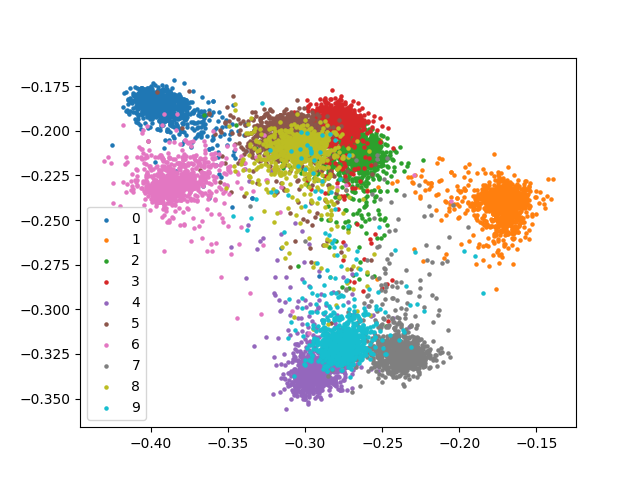
\includegraphics[width=0.9\linewidth]{siamese_more_pos}
				\end{center}
				\caption{Result of Siamese Network. The separation is fair. Some interesting substructure is notable (digit 4, 7 and 9; digit 2 and 3).\label{fig:siamese_more_pos}}
			\end{figure}
			
		\subsection{Triplet Network}
			The result of siamese network is shown in figure \ref{fig:triplet}. The 10 digits are separated very well. Digits 9, 7 and 4 are separated better and digits 2 and 3 are also well separated. Interestingly, we can see that the clusters of digit 9, 7 and 4 and digits 2 and 3 are still close to each other, which means the substructure is somewhat remained in the output.
			\begin{figure}[htbp]
				\begin{center}
					%\fbox{\rule{0pt}{2in} \rule{0.9\linewidth}{0pt}}
					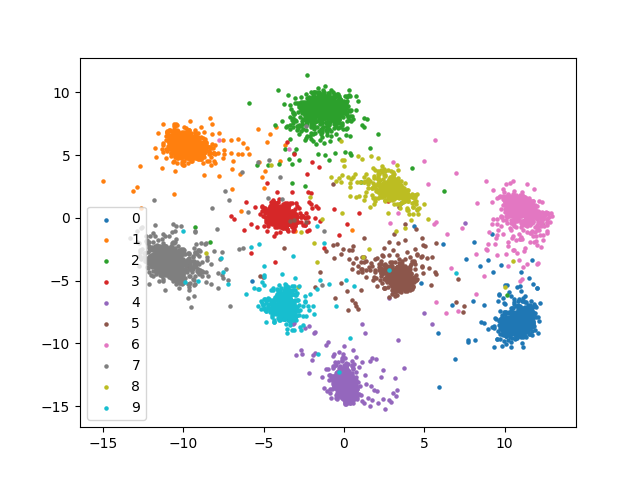
\includegraphics[width=0.9\linewidth]{triplet}
				\end{center}
				\caption{Result of Triplet Network.\label{fig:triplet}}
			\end{figure}
		\subsection{n-Tuple Network}
			We implement the original n-Tuple network using 10-tuples. However, the result in figure \ref{fig:fail_tuple} shows that the output points collapsed into one very little area.
			One possible reason could be that because the dot product is on points that are not normalized, all 0's could be a trivial solution of the problem.
			
				\begin{figure}[htbp]
					\begin{center}
						%\fbox{\rule{0pt}{2in} \rule{0.9\linewidth}{0pt}}
						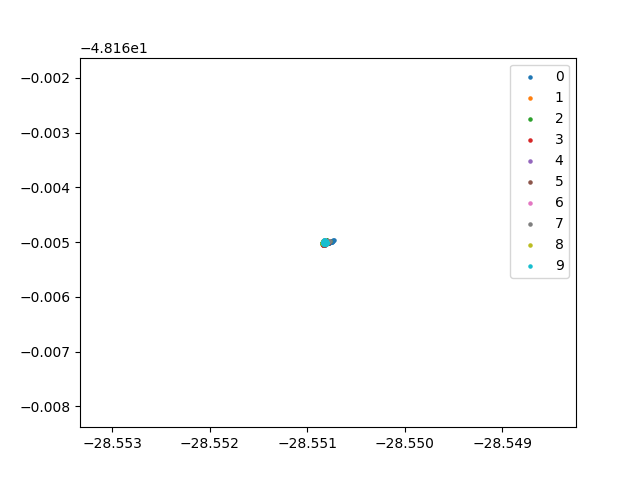
\includegraphics[width=0.9\linewidth]{fail_tuple}
					\end{center}
					\caption{Result of n-Tuple Network using 10-tuples. The points collapsed into a very little area.\label{fig:fail_tuple}}
				\end{figure}
			
			Several attempts have been made on restricting the norm of embeddings. While none of them shows better performance on metric learning. We adopt a solution described in the paper: Adding $L_2-$ norm for training embeddings in the loss function and this should not only constrain resulting embeddings in a reasonable range, but will also enhance convexity of the system.
			
			\begin{align}
			&L(\{x_i,x_i^+\}^N_{i=1})\notag\\
			=&\frac{1}{N}\log(\sum_{i=1}^N\exp(\sum_{j=1}^Ny^T_iy_j^+-y_i^Ty_i^+))+ \frac{\lambda}{2N} \sum_{i=1}^N(\lvert y_i\rvert^2+ \lvert y^+_i\rvert^2)
			\end{align}
			
			\begin{figure}[t]
				
				\begin{center}
					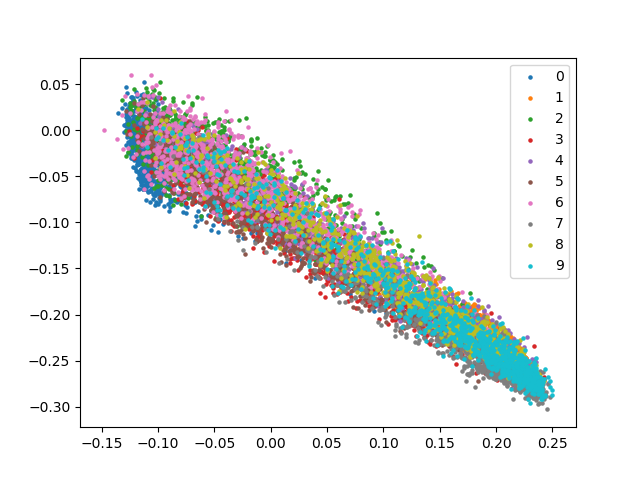
\includegraphics[width=0.5\linewidth]{fig1000}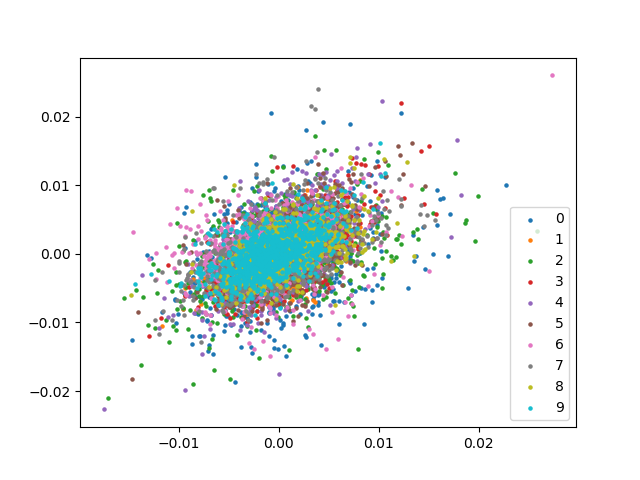
\includegraphics[width=0.5\linewidth]{fig600}
					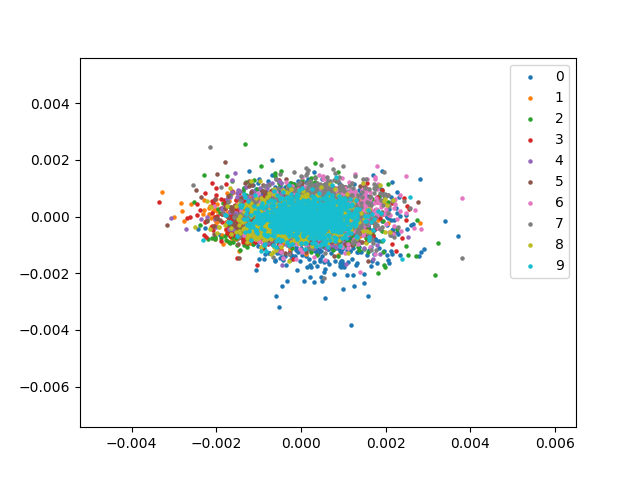
\includegraphics[width=0.5\linewidth]{fig2500}
					\caption{3-pair loss with constraint $\lambda (L_2)^2[\lambda=1.0]$ and $\lambda L_2[\lambda=1.0]$;10-pair loss with constraint $\lambda (L_2)^2[\lambda=1.0]$, and 10-pair sampling fails after long run}
					%\fbox{\rule{0pt}{2in} \rule{0.9\linewidth}{0pt}}
					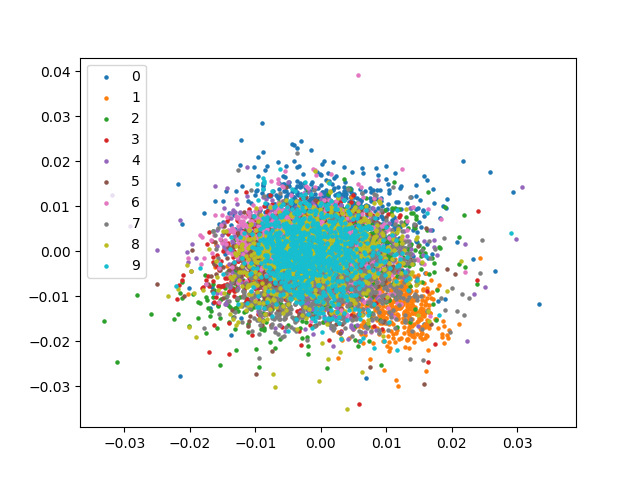
\includegraphics[width=0.9\linewidth]{fig150}
				\end{center}
				\caption{3-pair loss with $\lambda L_2$ constraint and weight $\lambda=0.3$.  We also added negative cutoff $m$ in equation \ref{eq:negative}, this proves improve the training result.}
				
				
				Another observation is that while optimizing contrastive loss and triplet loss is approachable for momentum optimizer, we could hardly optimize $(N+1)-$pair loss with it: it is harder to optimize $(N+1)-$pair loss. 
			\end{figure}
			
			Inspired by the loss function of Triplet Network, we abandoned the dot product loss function and designed two new loss functions for n-Tuple network. They have better performance but still failed to outperform Triplet Network.
			
			The first function is exactly the Triplet Network loss function using each two instances from the same class in the tuple as positive examples, and 9 instances from other classes as negative examples. The loss function turned out to be too complicated and TensorFlow uses significantly more time to construct the ``graph''. The result is shown in figure \ref{fig:first_tuple}. We can see mediocre separation of data from different classes. However, the scattering of data is in very weird pattern, which may be a result of highly dependent input data (90 triplets are produced by one 10-tuple which contains 20 instances). 
			
			\begin{figure}[htbp]
				\begin{center}
					%\fbox{\rule{0pt}{2in} \rule{0.9\linewidth}{0pt}}
					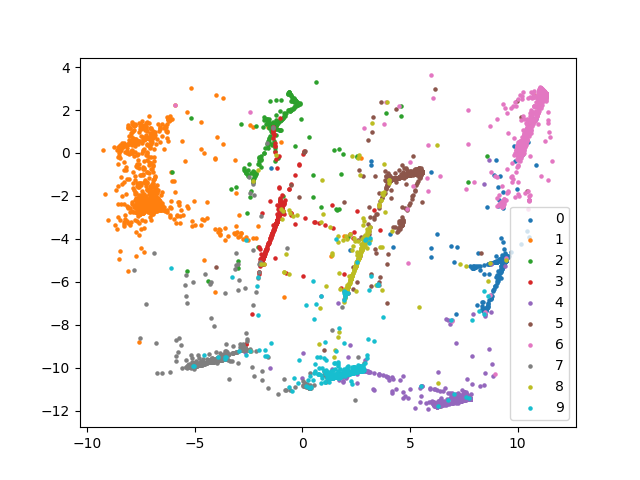
\includegraphics[width=0.9\linewidth]{first_tuple}
				\end{center}
				\caption{Result of n-Tuple Network using Triplet loss function. The separation is mediocre but the scattering of data is strange, which may caused by high dependency of input data.\label{fig:first_tuple}}
			\end{figure}
			
			The second function is a combined version of n-Tuple and Triplet loss function. We still use Euclidean distance in the function, but only produce 10 loss value per 10-tuple. In specific, we extract 2 instances from the same class in one tuple to form $y$ and $y+$ and choose other 9 as $y_-^i$'s. One loss value is defined as
			
			\begin{equation}
				\frac{\exp{(\lvert y-y_+ \rvert)}}{\exp{(\lvert y-y_+ \rvert)} + \sum_i\exp{(\lvert y-y_-^i \rvert)}}
			\end{equation}
			and the total loss is an average among the 10 loss values per tuple and also among 20 tuples. The result is shown in figure \ref{fig:second_tuple}. It can be observed that the scattering of data is more ``normal'', but only digit 0 and digit 6 has been better separated from the whole dataset.
			
			\begin{figure}[htbp]
				\begin{center}
					%\fbox{\rule{0pt}{2in} \rule{0.9\linewidth}{0pt}}
					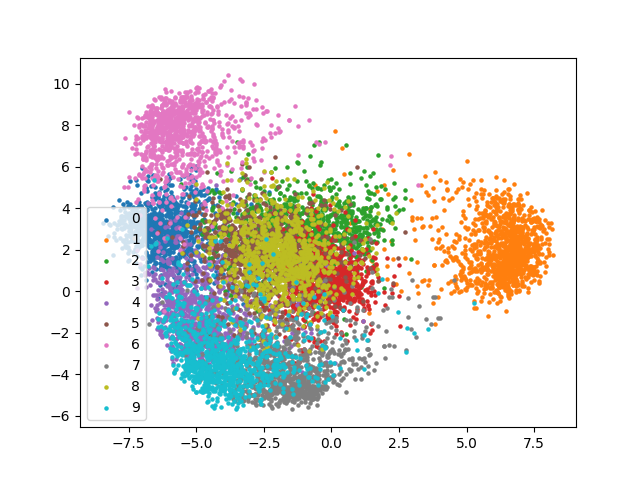
\includegraphics[width=0.9\linewidth]{second_tuple}
				\end{center}
				\caption{Result of n-Tuple network with combined loss function. The scattering of points looks more ``normal'' but has a worse separation.\label{fig:second_tuple}}
			\end{figure}
			
			The reason why the n-Tuple Network with Triplet Network loss function has a bad distribution may also be that the method is not able to reduce the dimensionality into 2. Instead, we try 20-dimensional network output and use unsupervised method to further reduce the dimensionality.
		\subsubsection{n-Tuple Network with PCA}
			PCA is the most classical unsupervised linear dimensionality reduction method. We feed our 20-dimensional output into PCA, and the result is shown in figure \ref{fig:first_tuple_pca}. We can observe that the distribution is better than the previous result shown in figure \ref{fig:first_tuple}. This suggests that this model is able to work when the required output if of more dimensions. 
			
			\begin{figure}[htbp]
				\begin{center}
					%\fbox{\rule{0pt}{2in} \rule{0.9\linewidth}{0pt}}
					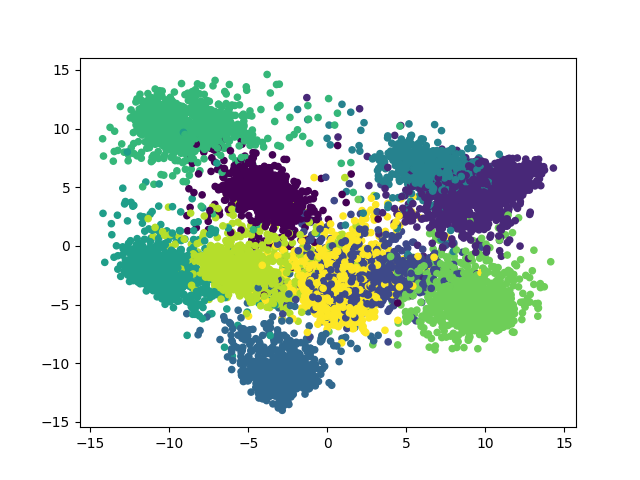
\includegraphics[width=0.9\linewidth]{first_tuple_pca}
				\end{center}
				\caption{Result of n-Tuple Network using Triplet loss function, which output 20-dimensional vectors, and then post-processed by PCA.\label{fig:first_tuple_pca}}
			\end{figure}
		\subsubsection{n-Tuple Network with t-SNE}
			There is no guarantee that the manifold in the high-dimensional space can be precisely shown by a linear method, PCA. Thus, we use t-SNE to retain more structures. t-SNE \cite{bengio2009learning} is a well-known unsupervised non-linear dimensionality reduction methods. We use t-SNE on the 20-dimensional output. The result is shown in \ref{fig:first_tuple_tsne}.
			
			\begin{figure}[htbp]
				\begin{center}
					%\fbox{\rule{0pt}{2in} \rule{0.9\linewidth}{0pt}}
					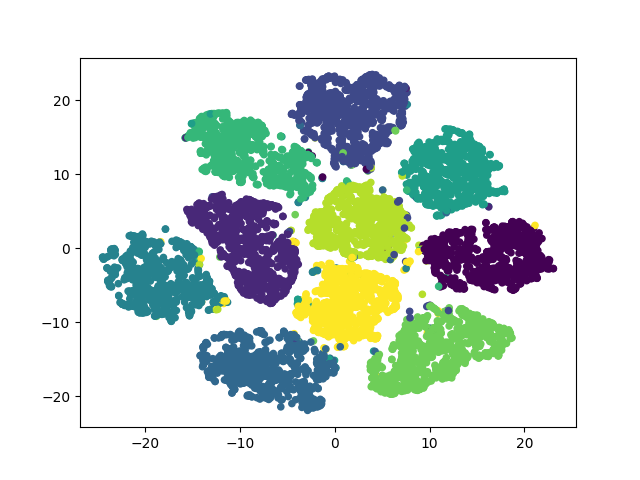
\includegraphics[width=0.9\linewidth]{first_tuple_tsne}
				\end{center}
				\caption{Result of n-Tuple Network using Triplet loss function, which output 20-dimensional vectors, and then post-processed by t-SNE.\label{fig:first_tuple_tsne}}
			\end{figure}
			
			We can compare our result against running t-SNE direct on the MNIST dataset reduced from $28\time 28$-dimensional images to $50$-dimensional vectors shown in figure \label{fig:tsne}. We can observe that the supervising information enhanced the performance of t-SNE. The examples from the same class is clustered more tightly. This phenomenon is more significant in the burn-in stage of t-SNE, which requires tighter clusters than the following steps. The result of it with our n-Tuple implementation is shown in figure \ref{fig:first_tuple_tsne_burnin}, where the points of each classes are clustered in to a small round area. In contrast, the t-SNE burn-in result using only the original dataset in image \ref{fig:tsne_burnin} shown that some classes are not well separable, and the shape of each cluster is also not round. This suggests that the supervised metric learning does create a better embedding for the data.
			
			\begin{figure}[htbp]
				\begin{center}
					%\fbox{\rule{0pt}{2in} \rule{0.9\linewidth}{0pt}}
					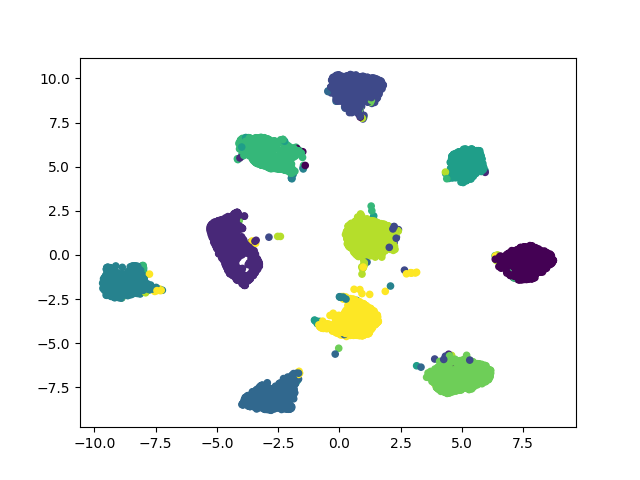
\includegraphics[width=0.9\linewidth]{first_tuple_tsne_burnin}
				\end{center}
				\caption{Burn-in result of t-SNE, with n-Tuple.\label{fig:first_tuple_tsne_burnin}}
			\end{figure}

			\begin{figure}[htbp]
				\begin{center}
					%\fbox{\rule{0pt}{2in} \rule{0.9\linewidth}{0pt}}
					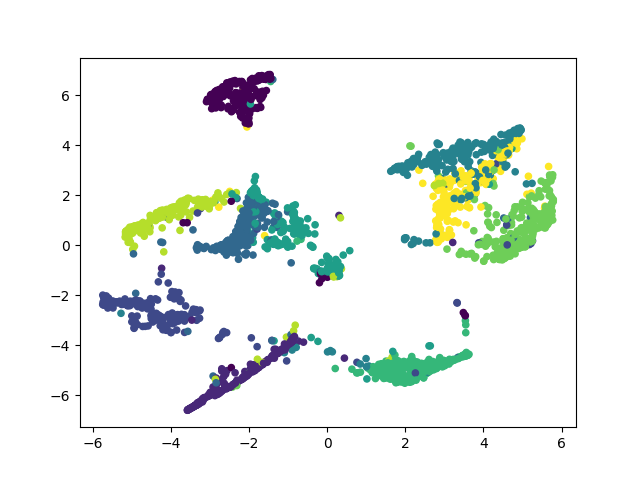
\includegraphics[width=0.9\linewidth]{tsne_burnin}
				\end{center}
				\caption{Burn-in result of t-SNE, on original dataset.\label{fig:tsne_burnin}}
			\end{figure}
	\section{Furture work}
	In addition to the contrastive, triplet and $(N+1)$-tuple embeddings in this report. Another pratical embedding in literature one should notice is the lifted structure embedding. We also takes $N$ samples as a training group. In lifted structure approach training batch to be not completely random as $(N+1)$ tuple sampling, but integrate elements of importance sampling: choosing positive elements and random and generate "important" negative samples oriented to the positive examples. This is intuitive in the sense that when seeing squared loss as repulsive harmonic potentials, we can push apart "important" negative pairs. 
				\begin{figure}[t]
				
				\begin{center}
					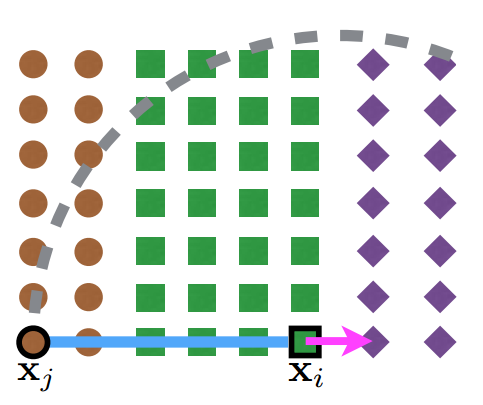
\includegraphics[width=0.5\linewidth]{constrastiveDemo}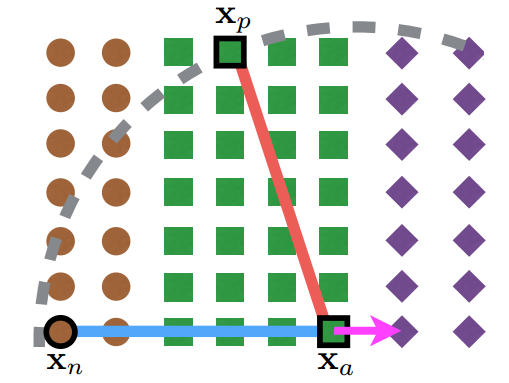
\includegraphics[width=0.5\linewidth]{tripletDemo}
					\caption{Constrastive Sampling and Triplet Sampling}
					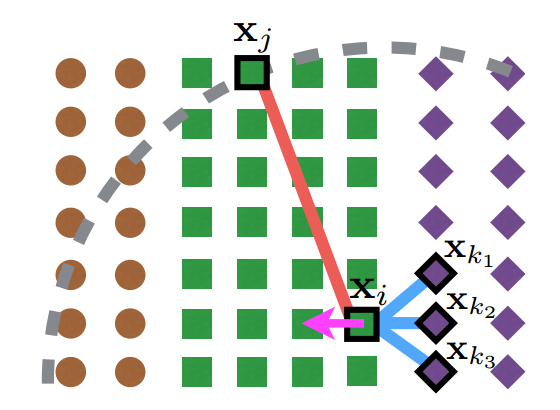
\includegraphics[width=0.5\linewidth]{liftedDemo}
					\caption{Lifted Structured Feature Embedding, sampling oriented to the positive samples\label{fig:lift}}
					%\fbox{\rule{0pt}{2in} \rule{0.9\linewidth}{0pt}}
				\end{center}
			Deep Metric Learning via Lifted Structured Feature Embedding (In this section, figures are from original paper \cite{lifted}) 
			\end{figure}

	The sampling method is intuitive in the sense that it takes full advantage of the training batches in the neural network training by lifting the vector of pairwise distances within the batch to the matrix of pairwise distances. Figure \ref{fig:lift} gives an illustration. 

	As suggested in paper \cite{lifted}, sampling negative examples oriented to the positive instance, the training is done on the loss function 
	\begin{equation}
		L=\frac{1}{|\mathcal{P}|}\sum_{(i,j)\in \mathcal{P}}\max(0, L_{i,j})
	\end{equation}
	where
	\begin{equation}
		L_{i,j}=\max\{\max_{(i,k)\in\mathcal{N}}\alpha-D_{i,k}, \max_{(j,l)\in\mathcal{N}}\alpha-D_{j,l}\}+D_{i,j}\label{eq:leftij}
	\end{equation}
	and $\mathcal{P}$ and $\mathcal{N}$ are sampled postive and negative pairs with $D$.current step metric. And due to non-convexity in \ref{eq:leftij}, the training should be tricky\cite{lifted}.
	\section{Conclusion \label{sec:Conc}}
		We have implemented a backend for experimenting metric learning methods. We experimented three frameworks, Siamese Network, Triplet Network and n-Tuple Network on MNIST dataset. Siamese Network shows a fair performance while Triplet Network outperforms Siamese as expected. However, the original n-Tuple Network does not work in our experiments and our modification on the loss function gives a partly work version.
	{\small
		\bibliographystyle{ieee}
		\bibliography{egbib}
	}
	
\end{document}
